\documentclass[paper=a4, open=any]{scrbook}

\usepackage[hang]{caption}
\usepackage{microtype, textcomp}
\usepackage[intlimits]{mathtools}
\usepackage{amsfonts, amssymb, longtable, array, tabu, scrlayer-scrpage}
\usepackage[per-mode=fraction, locale=DE, detect-all=true]{siunitx}
\usepackage{unicode-math, icomma}
\usepackage{fontspec}
\usepackage{polyglossia}
\setdefaultlanguage[spelling=new]{german}
\usepackage[autostyle]{csquotes}
\usepackage[margin=20mm, bottom=15mm, includefoot]{geometry}
\usepackage{graphicx, xcolor}
\usepackage[unicode=true, colorlinks=false, breaklinks=true, pdfborder={0 0 0}]{hyperref}
\usepackage{bookmark}

\newcommand{\origttfamily}{}
\let\origttfamily=\ttfamily
\renewcommand{\ttfamily}{\origttfamily \hyphenchar\font=`\-}
\setmainfont{Tex Gyre Termes}
\setmathfont{Tex Gyre Termes Math}
\setmathfont{TeX Gyre Termes}[range=\mathup/{latin,Latin,num}]
\setsansfont{Latin Modern Sans}[Scale=MatchLowercase]
\setmonofont{LMMonoLt10-Bold}[Scale=MatchLowercase]
\AtBeginDocument{%
	\let\umathpi\pi%ersatzbefehl für kursives pi
	\renewcommand\pi{\symup\umathpi}%alle \pi per default aufrecht
}
\newfontfamily\Commons{Commons}
\newfontfamily\Gost{Gost}
\defaultfontfeatures{Ligatures=TeX}

\title{Aufbauanleitung FUOCO STEP}
\author{Felix Pflaum}
\date{31.05.2018}

\begin{document}
	\begin{titlepage}
		\vspace*{\fill}
		\begin{center}
			\includegraphics[width=\textwidth]{logo}
		\end{center}
		\vfill
		\begin{center}{\fontsize{40pt}{40pt} \Commons{Aufbau- und Bedienungsanleitung}} \\ \vfill
			{\fontsize{24pt}{24pt} \Gost{Felix Pflaum}}
		\end{center}
		\vfill
	\end{titlepage}
	\part{Aufbauanleitung}
		\chapter{Vorbemerkungen}
			FUOCO STEP besteht aus zwei Platinen (=PCBs), der Basis (kleine Platine) und dem Panel (große Platine), zum Lieferumfang des Bausatzes gehören neben den Platinen und ihren Lötteilen, die in den Tabellen in den jeweiligen Unterkapiteln aufgeführt wurden:
			\begin{itemize}
				\item Koffer Seahorse SE-120
				\item Blei-Gel-Akku \SI{12}{\volt}/\SI{1,2}{\ampere\hour}
				\item Hauptschalter mit blauer LED
				\item Spannungsanzeige
				\item Micro-USB-Anschluss für Gehäusemontage
				\item Schlüsselschalter
				\item Druckschalter für Durchgangstest
				\item Drehschalter mit elf Widerständen und drei Kabeln (rot, weiß, schwarz)
				\item Crimpbuchse mit drei Kabeln (rot, weiß, grau)
				\item Crimpbuchse mit acht Kabeln (blau, schwarz, rot, schwarz, violett, violett, gelb, gelb)
				\item Je ein rotes und ein schwarzes Kabel mit und ohne Kabelschuh (insg. vier Kabel)
				\item Ein Paar Deans-Steckverbinder (Buchse für Anschluss an Batterie, Stecker an PCB)
				\item Vier Gewindeschrauben M3x16 mit Muttern
				\item Zwei Gewindeschrauben M3x10 mit Muttern
				\item Zwei Gewindeschrauben M2x6 mit Muttern
				\item Sechs Blechschrauben 3x10
				\item Schrumpfschlauchabschnitte in \SI{26}{\milli\metre}, \SI{6,4}{\milli\metre} und \SI{3,2}{\milli\metre}
				\item Isolationsabdeckung für Lötkontakte
			\end{itemize}

			\section{Benötigtes Werkzeug}
				Für den Aufbau braucht man:
				\begin{itemize}
					\item Lötkolben
					\item Lötzinn
					\item Seitenschneider
					\item Kreuzschraubendreher PH1 oder PZ1
					\item Zange oder Maulschlüssel zum Festhalten/Drehen von Muttern
					\item Heißluftfön zum Schrumpfen von Schrumpfschläuchen
					\item Gewebeband
					\item Entlötlitze und -pumpe können sich für die Fehlerkorrektur als hilfreich erweisen, sind aber nicht zwingend notwendig
				\end{itemize}

			\section{Wichtige Hinweise}
				Wenig ist frustrierender als harte Arbeit, die man umsonst verrichtet, vom im wahrsten Sinne des Wortes verbrannten Geld bei Zerstörung von Platine oder Bauteilen ganz zu schweigen. Daher bitte beachten:
				\begin{itemize}
					\item Beim Löten gewissenhaft und gründlich arbeiten. Auf eine saubere Trennung der Lötstellen achten, speziell bei enger Nachbarschaft (Stift- und Buchsenleisten, integrierte Schaltungen, \dots).
					\item Mit wenigen Ausnahmen muss die Bauteilorientierung entweder aus Platz- oder Funktionsgründen beachtet werden. Daher erst genau schauen, dann löten, denn gerade bei den integrierten Schaltungen mit vier oder mehr Kontakten ist ein nachträgliches Auslöten ziemlich kompliziert und führt häufig zu Schäden an Bauteil und/oder Platine. Verpolte Elektrolytkondensatoren können zudem sehr spektakulär explodieren und das wollen wir doch lieber den pyrotechnischen Gegenständen überlassen!
					\item Vor dem Anschließen des Akkus an die Platine noch einmal kritisch prüfen, dass man keine unerwünschten Verbindungen hergestellt hat. Der Akku liefert für einige Sekunden problemlos Strom im zweistelligen Amperebereich, für die manche Bauteile und Leiterzüge nicht ausgelegt sind.
				\end{itemize}
		\chapter{Aufbau}
			\section{Panel}

				\subsection*{Bauteilindex}

					Die in der Platine zu verlötenden Teile sind in der folgenden Tabelle aufgeführt:

					\begin{longtabu}
						to \textwidth[l]{lX[-1]X}
						Reference & Value/Name             & Package                            \\ \hline\hline
						\endhead
						CH        &                        &                                    \\*
						CH1       & CH                     & LMZFL\_7-2-135-3.5                 \\
						CH2       & CH                     & LMZFL\_7-2-135-3.5                 \\
						CH3       & CH                     & LMZFL\_7-2-135-3.5                 \\
						CH4       & CH                     & LMZFL\_7-2-135-3.5                 \\
						CH5       & CH                     & LMZFL\_7-2-135-3.5                 \\
						CH6       & CH                     & LMZFL\_7-2-135-3.5                 \\
						CH7       & CH                     & LMZFL\_7-2-135-3.5                 \\
						CH8       & CH                     & LMZFL\_7-2-135-3.5                 \\
						CH9       & CH                     & LMZFL\_7-2-135-3.5                 \\
						CH10      & CH                     & LMZFL\_7-2-135-3.5                 \\
						CH11      & CH                     & LMZFL\_7-2-135-3.5                 \\
						CH12      & CH                     & LMZFL\_7-2-135-3.5                 \\
						CH13      & CH                     & LMZFL\_7-2-135-3.5                 \\
						CH14      & CH                     & LMZFL\_7-2-135-3.5                 \\
						CH15      & CH                     & LMZFL\_7-2-135-3.5                 \\
						CH16      & CH                     & LMZFL\_7-2-135-3.5                 \\
						\hline

						D         &                        &                                    \\*
						D1        & LED                    & LED\_D3.0mm                        \\
						D2        & LED                    & LED\_D3.0mm                        \\
						D3        & LED                    & LED\_D3.0mm                        \\
						D4        & LED                    & LED\_D3.0mm                        \\
						D5        & LED                    & LED\_D3.0mm                        \\
						D6        & LED                    & LED\_D3.0mm                        \\
						D7        & LED                    & LED\_D3.0mm                        \\
						D8        & LED                    & LED\_D3.0mm                        \\
						D9        & LED                    & LED\_D3.0mm                        \\
						D10       & LED                    & LED\_D3.0mm                        \\
						D11       & LED                    & LED\_D3.0mm                        \\
						D12       & LED                    & LED\_D3.0mm                        \\
						D13       & LED                    & LED\_D3.0mm                        \\
						D14       & LED                    & LED\_D3.0mm                        \\
						D15       & LED                    & LED\_D3.0mm                        \\
						D16       & LED                    & LED\_D3.0mm                        \\
						D17       & ACTIVE                 & LED\_D5.0mm                        \\
						D18       & TRIGGERED              & LED\_D5.0mm                        \\
						D19       & ARMED                  & LED\_D5.0mm                        \\
						D20       & DATA                   & LED\_D5.0mm                        \\
						\hline

						J         &                        &                                    \\*
						J1        & Conn\_02x22\_Odd\_Even & PinHeader\_2x22\_P2.54mm\_Vertical \\
						\hline

						TR        &                        &                                    \\*
						TR1       & CH                     & LMZFL\_7-2-135-3.5                 \\
						\hline
					\end{longtabu}

				\subsection*{Vorgehensweise}
					Die Bauteile sollten von klein nach groß eingelötet werden und jeweils bündig auf der Platine aufliegen:
					\begin{enumerate}
						\item Die 3-mm-LEDs, hierbei ist auf korrekte Polarität zu achten: Der kürzere Draht an der abgeflachten Seite der LED gehört ins quadratische Lötpad, der längere Draht ins runde. Drähte nach dem Einlöten kürzen.
						\item Die 5-mm-LEDs, hier analog zu den 3-mm-LEDs vorgehen. Die Farbzuordnung lautet:
								\begin{itemize}
									\item ARMED: rot
									\item DATA: geld
									\item ACTIVE: orange
									\item TRIGGERED: grün
								\end{itemize}
								Drähte nach dem Einlöten kürzen.
						\item Die Klemmen
						\item Die Stiftleiste, die im Gegensatz zu den anderen Bauteilen von der Unterseite zu stecken und von der Oberseite zu löten ist
					\end{enumerate}

					Der Zwischenstand sollte dann in etwa so aussehen (LEDs nicht farbecht!): \\
					\begin{center}
						\includegraphics[width=.9\textwidth]{panel3d}
					\end{center}

					Anschließend müssen die restlichen Löcher in der Platine gefüllt werden:

					\begin{description}
						\item[Drehschalter] Die Schritte zur Konfektionierung des Drehschalters sind in folgender Graphik illustriert, den Schalter hierzu kopfüber positionieren, um bequem an der Unterseite arbeiten zu können:
						\begin{center}
							\includegraphics[width=.8\textwidth]{Drehschalter}
							\captionof{figure}{Konfektionierung des Drehschalters: Stecken der Widerstände, Verlöten der Widerstände, Verlöten der Kabel, Isolierung mittels Schrumpfschlauch (von links oben nach rechts unten)}
						\end{center}
						Zunächst müssen die elf kleinen Widerstände von innen nach außen zwischen den Kontakten 1 und 2, 2 und 3, 3 und 4, \dots, 11 und 12 gesteckt werden, rur die Lücke zwischen 1 und 12 bleibt frei (Bild links oben). Anschließend werden die Drahtpaare an den Pins 2 bis 11 gelötet; 1, 12 noch nicht verlöten, erst Kabel anbringen (Bild rechts oben). Am Pin 1 ist das kurze schwarze, am Pin 12 das kurze rote und zusätzlich am inneren Pin das kurze gelbe Kabel anzulöten (Bild links unten). Anschließend den grünen Schrumpfschlauch auf den Schalter ziehen und per Fön erhitzen, wobei die Kabel noch herausstehen sollen (Bild rechts unten).  
						
						Nun den Schalter in die Platine stecken, festschrauben und die Schalterkappe befestigen. Am Ende müssen dann die drei Kabel auf der Platine festgelötet werden. Hierzu zunächst die Pads kräftig mit Lötzinn vorverzinnen, die Kabel am Ende der Isolierung abknicken, Pad erhitzen und Kabelende in den Zinn drücken: rot bei Pad \enquote{3,3V}, gelb bei Pad \enquote{ADC} und schwarz bei Pad \enquote{GND}.
						\item [Testschalter] In die Platine stecken und festschrauben
						\item [Schlüsselschalter] In die Platine stecken und festschrauben, dabei darauf achten, dass der rote Punkt am Schalter bei \enquote{Inactive}, der grüne bei \enquote{Armed} liegt.
						\item [Ladebuchse] Den mittleren Kontakt auf der Unterseite abzwicken, dann in die Platine stecken und festschrauben
						\item [Spannungsanzeige] In die Platine stecken und mit dem M2-Schrauben und zugehörigen Muttern festschrauben
						\item [Hauptschalter] In die Platine stecken, bis er einrastet
						\item [Micro-USB-Anschluss] Mit den zugehörigen Schrauben festschrauben
						\item [Abdeckung der Lötstellen] Mit den beiden M3x10-Schrauben und passenden Muttern befestigen
					\end{description}

					Die Bedien- und Anzeigeelemente, welche in der Platine verschraubt sind, müssen nun noch mit den entsprechenden Kabeln verbunden werden, die später den Kontakt zur Steuerplatine herstellen.

					Beim dreipoligen Crimpgehäuse zunächst Schrumpfschlauchstücke über die losen Kabelenden bis zum Gehäuse schieben und folgendermaßen verlöten: Rotes Kabel an den äußeren silbernen Kontakt des Hauptschalters, weißes Kabel an den Mittelkontakt und graues Kabel an den goldenen Kontakt. Kontakte danach mit den vorher aufgeschobenen Schrumpfschläuchen isolieren.

					Auch beim achtpoligen Crimpgehäuse zunächst Schrumpfschläuche über die losen Kabelenden bis zum Gehäuse schieben und folgendermaßen verlöten: Rotes dickes Kabel an den Mittelkontakt der Ladebuchse, schwarzes dickes Kabel an den Außenkontakt. Das dünne blaue Kabel muss mit den beiden inneren Kontakten des Displays verbunden werden, das dünne schwarze Kabel mit dem Außenkontakt (siehe Bild):
					
					Die beiden violetten Kabel an den Schlüsselschalter, die beiden gelben Kabel an den Testschalter löten. Kontakte anschließend mit Schrumpfschlauch isolieren.

					\newpage
			\section{Basis}
				\subsection*{Bauteilindex}

					Die in der Platine zu verlötenden Teile sind in der folgenden Tabelle aufgeführt:

					\begin{longtabu}
						to \textwidth[l]{lX[-1]X}
						Reference & Value/Name             & Package                                                 \\ \hline\hline
						\endhead
						C         &                        &                                                         \\*
						C1        & 100n                   & C\_Disc\_D3.8mm\_W2.6mm\_P2.50mm                        \\
						C2        & 100n                   & C\_Disc\_D3.8mm\_W2.6mm\_P2.50mm                        \\
						C3        & 100n                   & C\_Disc\_D3.8mm\_W2.6mm\_P2.50mm                        \\
						C4        & 100n                   & C\_Disc\_D3.8mm\_W2.6mm\_P2.50mm                        \\
						C5        & 100n                   & C\_Disc\_D3.8mm\_W2.6mm\_P2.50mm                        \\
						C6        & 100n                   & C\_Disc\_D3.8mm\_W2.6mm\_P2.50mm                        \\
						C7        & 100n                   & C\_Disc\_D3.8mm\_W2.6mm\_P2.50mm                        \\
						C8        & 100n                   & C\_Disc\_D3.8mm\_W2.6mm\_P2.50mm                        \\
						C9        & 10u                    & CP\_Radial\_D6.3mm\_P2.50mm                             \\
						C10       & 10u                    & CP\_Radial\_D6.3mm\_P2.50mm                             \\
						C11       & 100n                   & C\_Disc\_D3.8mm\_W2.6mm\_P2.50mm                        \\
						C12       & 100n                   & C\_Disc\_D3.8mm\_W2.6mm\_P2.50mm                        \\
						C13       & 4m7                    & CP\_Radial\_D18.0mm\_P7.50mm                            \\
						C14       & 4m7                    & CP\_Radial\_D18.0mm\_P7.50mm                            \\
						C15       & 100n                   & C\_Disc\_D3.8mm\_W2.6mm\_P2.50mm                        \\
						\hline

						D         &                        &                                                         \\*
						D1        & 1N4001                 & D\_DO-41\_SOD81\_P10.16mm\_Horizontal                   \\
						D2        & 1N4001                 & D\_DO-41\_SOD81\_P10.16mm\_Horizontal                   \\
						\hline

						J         &                        &                                                         \\*
						J1        & Conn\_02x22\_Odd\_Even & PinSocket\_2x22\_P2.54mm\_Vertical                      \\
						J2        & Conn\_01x03            & Molex\_KK-254\_AE-6410-03A\_1x03\_P2.54mm\_Vertical     \\
						J3        & Conn\_01x08            & Molex\_KK-254\_AE-6410-08A\_1x08\_P2.54mm\_Vertical     \\
						\emph{J4} & Conn\_01x05            & PinHeader\_1x05\_P2.54mm\_Vertical                      \\
						\emph{J5} & Conn\_02x05\_Odd\_Even & IDC-Header\_2x05\_P2.54mm\_Vertical                     \\
						\emph{J6} & Conn\_01x02            & PinHeader\_1x02\_P2.54mm\_Vertical                      \\
						\emph{J7} & USB\_B\_Micro          & MIUSB-F5MX-BB-U                                         \\
						\hline

						Q         &                        &                                                         \\*
						Q1        & IRF3708                & TO-220-3\_Vertical                                      \\
						Q2        & IRF3708                & TO-220-3\_Vertical                                      \\
						Q3        & IRF3708                & TO-220-3\_Vertical                                      \\
						Q4        & IRF3708                & TO-220-3\_Vertical                                      \\
						Q5        & IRF3708                & TO-220-3\_Vertical                                      \\
						Q6        & IRF3708                & TO-220-3\_Vertical                                      \\
						Q7        & IRF3708                & TO-220-3\_Vertical                                      \\
						Q8        & IRF3708                & TO-220-3\_Vertical                                      \\
						Q9        & IRF3708                & TO-220-3\_Vertical                                      \\
						Q10       & IRF3708                & TO-220-3\_Vertical                                      \\
						Q11       & IRF3708                & TO-220-3\_Vertical                                      \\
						Q12       & IRF3708                & TO-220-3\_Vertical                                      \\
						Q13       & IRF3708                & TO-220-3\_Vertical                                      \\
						Q14       & IRF3708                & TO-220-3\_Vertical                                      \\
						Q15       & IRF3708                & TO-220-3\_Vertical                                      \\
						Q16       & IRF3708                & TO-220-3\_Vertical                                      \\
						Q17       & BC337                  & TO-92\_Inline\_Wide                                     \\
						Q18       & IRF4905                & TO-220-3\_Vertical                                      \\
						Q19       & BC337                  & TO-92\_Inline\_Wide                                     \\
						Q20       & BC327                  & TO-92\_Inline\_Wide                                     \\
						\hline

						R         &                        &                                                         \\*
						R1        & 10k                    & R\_Axial\_DIN0207\_L6.3mm\_D2.5mm\_P10.16mm\_Horizontal \\
						R2        & 4k7                    & R\_Axial\_DIN0207\_L6.3mm\_D2.5mm\_P10.16mm\_Horizontal \\
						R3        & 150                    & R\_Radial\_Power\_L9.0mm\_W10.0mm\_Px2.90mm\_Py2.40mm   \\
						R4        & 2R2                    & R\_Radial\_Power\_L9.0mm\_W10.0mm\_Px2.90mm\_Py2.40mm   \\
						R5        & 1k0                    & R\_Axial\_DIN0207\_L6.3mm\_D2.5mm\_P10.16mm\_Horizontal \\
						R6        & 270                    & R\_Axial\_DIN0207\_L6.3mm\_D2.5mm\_P10.16mm\_Horizontal \\
						R7        & 1k0                    & R\_Axial\_DIN0207\_L6.3mm\_D2.5mm\_P10.16mm\_Horizontal \\
						R8        & 1k0                    & R\_Axial\_DIN0207\_L6.3mm\_D2.5mm\_P10.16mm\_Horizontal \\
						R9        & 330                    & R\_Axial\_DIN0207\_L6.3mm\_D2.5mm\_P10.16mm\_Horizontal \\
						R10       & 150k                   & R\_Axial\_DIN0207\_L6.3mm\_D2.5mm\_P10.16mm\_Horizontal \\
						R11       & 47k                    & R\_Axial\_DIN0207\_L6.3mm\_D2.5mm\_P10.16mm\_Horizontal \\
						R12       & 1k0                    & R\_Axial\_DIN0207\_L6.3mm\_D2.5mm\_P10.16mm\_Horizontal \\
						R13       & 1k0                    & R\_Axial\_DIN0207\_L6.3mm\_D2.5mm\_P10.16mm\_Horizontal \\
						R14       & 1k0                    & R\_Axial\_DIN0207\_L6.3mm\_D2.5mm\_P10.16mm\_Horizontal \\
						R15       & 1k0                    & R\_Axial\_DIN0207\_L6.3mm\_D2.5mm\_P10.16mm\_Horizontal \\
						R16       & 47                     & R\_Radial\_Power\_L9.0mm\_W10.0mm\_Px2.90mm\_Py2.40mm   \\
						\hline

						RN        &                        &                                                         \\*
						RN1       & 10k                    & R\_Array\_SIP9                                          \\
						RN2       & 10k                    & R\_Array\_SIP9                                          \\
						RN3       & 4k7                    & R\_Array\_SIP9                                          \\
						RN4       & 4k7                    & R\_Array\_SIP9                                          \\
						\hline

						U         &                        &                                                         \\*
						U1        & ATmega328P-PU          & DIP-28\_W7.62mm                                         \\
						U2        & 74HC595                & DIP-16\_W7.62mm                                         \\
						U3        & 74HC595                & DIP-16\_W7.62mm                                         \\
						U4        & LM1084-3.3             & TO-220-3\_Vertical                                      \\
						U5        & SFH620A-3              & DIP-4\_W7.62mm                                          \\
						U6        & MCP6002-xP             & DIP-8\_W7.62mm                                          \\
						U7        & MCP2221\_IP            & DIP-14\_W7.62mm                                         \\
						U8        & XL6009\_Module         & XL6009\_STEP-UP-MODULE                                  \\
						\hline
					\end{longtabu}

				\subsection*{Vorgehensweise}
					Die Bauteile sollten auch hier von klein nach groß eingelötet werden und jeweils bündig auf der Platine aufliegen, sofern nichts anderes vermerkt ist:
					\begin{enumerate}
						\item Die kleinen Widerstände \texttt{R1}, \texttt{R2}, \texttt{R5}, \texttt{R6}, \texttt{R7}, \texttt{R8}, \texttt{R9}, \texttt{R10}, \texttt{R11}, \texttt{R12}, \texttt{R13}, \texttt{R14}, \texttt{R15} in der Bauform 0207, hier spielt die Polarität keine Rolle, allerdings ist auf die Werte zu achten, die anhand der Farbringe festgestellt werden können\footnote{Falls sich jemand genauer für die Kennzeichnung der Widerstände interessiert: jede Farben symbolisiert eine Zahl, nämlich schwarz=0, braun=1, rot=2, orange=3, gelb=4, grün=5, blau=6, violett=7, grau=8, weiß=9. Der Widerstandswert in Ohm ist bei fünf Ringen folgendermaßen zu lesen: (100*Ring1 + 10*Ring2 + Ring3) * 10$^{\text{Ring4}}$ mit einer Toleranz von Ring5, wobei bei Ring 5 braun=\SI{1}{\percent}, rot=\SI{2}{\percent}, grün=\SI{0,5}{\percent}, blau=\SI{0,25}{\percent}, violett=\SI{0,1}{\percent}, gold=\SI{5}{\percent} und silber=\SI{10}{\percent} bedeutet. Gold und silber können auch als Farben des Toleranzrings 4 auftreten, gold=-1, silber=-2. Der kleinste darstellbare Widerstandswert größer \SI{0}{\ohm} mit 1-\%-Toleranz wäre also die Kombination schwarz-schwarz-braun-silber-braun, dies entspricht \SI{0,01}{\ohm}, der größte so darstellbare Wert wäre weiß-weiß-weiß-weiß-braun, also \SI{999}{\giga\ohm}.}. Der erste Ring ist derjenige, der am weitesten außen am Gehäuse angebracht ist, ansonsten den Widerstand so drehen, dass die Farbreihenfolge einer in der Tabelle genannten entspricht, rechts muss immer ein brauner Ring sein. Besondere Vorsicht ist bei den Werten geboten, die sich nur um eine Zehnerpotenz, also nur im vierten Ring unterschieden!

								\begin{center}
									\begin{tabu}
										{|r@{\,}l|ccccc|}\hline
										\multicolumn{2}{|c|}{Wert} & 1. Ring        & 2. Ring              & 3. Ring               & 4. Ring & 5. Ring                                   \\ \hline\hline
										270                        & \si{\ohm}      & \color{red}rot       & \color{violet}violett & schwarz & schwarz              & \color{brown}braun \\ \hline
										330                        & \si{\ohm}      & \color{orange}orange & \color{orange}orange  & schwarz & schwarz              & \color{brown}braun \\ \hline
										1                          & \si{\kilo\ohm} & \color{brown}braun   & schwarz               & schwarz & \color{brown}braun   & \color{brown}braun \\ \hline
										4,7                        & \si{\kilo\ohm} & \color{yellow}gelb   & \color{violet}violett & schwarz & \color{brown}braun   & \color{brown}braun \\ \hline
										10                         & \si{\kilo\ohm} & \color{brown}braun   & schwarz               & schwarz & \color{red}rot       & \color{brown}braun \\ \hline
										47                         & \si{\kilo\ohm} & \color{yellow}gelb   & \color{violet}violett & schwarz & \color{red}rot       & \color{brown}braun \\ \hline
										150                        & \si{\kilo\ohm} & \color{brown}braun   & \color{green}grün     & schwarz & \color{orange}orange & \color{brown}braun \\ \hline
									\end{tabu}
								\end{center}
								Drähte nach dem Einlöten kürzen.

						\item Die beiden Dioden \texttt{D1} und \texttt{D2}, wobei die Orientierung wichtig ist. Drähte nach dem Einlöten kürzen.
						\item Die kleinen 100-nF-Kondensatoren \texttt{C1}, \texttt{C2}, \texttt{C3}, \texttt{C4}, \texttt{C5}, \texttt{C6}, \texttt{C7}, \texttt{C8}, \texttt{C11}, \texttt{C12}, \texttt{C15}, Orientierung spielt keine Rolle. Drähte nach dem Einlöten kürzen.
						\item Den ATmega328P-PU, die beiden 74HC595, den SFH620A-3, den MCP6002 und den MCP2221-I-P, dabei auf korrekte Orientierung achten. Die größeren Gehäuse besitzen an einer der kurzen Seiten eine halbkreisförmige Vertiefung, die im Bestückungsdruck auf der Platine nachempfunden ist, beim Optokoppler~(U5) ist Pin~1 durch einen Punkt auf dem Gehäuse markiert und gehört ins quadratische der vier Pads.
						\item Die Buchsenleiste, die im Gegensatz zu den anderen Bauteilen von der Unterseite zu stecken und von der Oberseite zu löten ist
						\item Die Widerstandsnetzwerke (RN), der Punkt auf dem schwarzen Gehäuse muss jeweils am quadratischen Lötpad liegen
						\item Die drei Transistoren \texttt{Q17}, \texttt{Q19} und \texttt{Q20} im Package TO-92. Orientierung beachten und nicht mit Gewalt in die Platine drücken. Es sollen ruhig noch ein paar Millimeter Draht auf der Oberseite herausschauen, das schwarze Gehäuse soll nicht aufliegen. Drähte nach dem Einlöten kürzen.
						\item Die Molexkonnektoren \texttt{J2} und \texttt{J3}, die Plastikwand muss jeweils zur Platinenmitte weisen
						\item Das Boost-Modul \texttt{U8}, Beschriftung auf dem Modul mit Beschriftung auf der Platine abgleichen!
						\item Die Elektrolytkondensatoren \texttt{C9} und \texttt{C10}, der Draht an der weißen Markierung am Gehäuse muss jeweils in das Loch im weißen Bereich.  Drähte nach dem Einlöten kürzen.
						\item Die Feldeffekttransistoren \texttt{Q1} bis \texttt{Q16} und \texttt{Q18} (Vorsicht, Q18 ist ein anderes Modell als die 16 anderen Transistoren!), auf korrekte Orientierung und Beschriftung achten. Beinchen nach dem Einlöten kürzen.
						\item Der Spannungsregler \texttt{U4}, auf korrekte Orientierung achten. Beinchen nach dem Einlöten kürzen.
						\item Die großen Zementwiderstände -- die Werte der Widerstände sind auf dem Gehäuse aufgedruckt; darauf achten, die richtigen Werte an der richtigen Stelle einzulöten.  Drähte nach dem Einlöten kürzen.
						\item Die großen 4700-\si{\micro\farad}-Kondensatoren \texttt{C13} und \texttt{C14}, der Draht an der weißen \enquote{-}-Markierung am Gehäuse muss jeweils in das Loch im weißen Bereich. Drähte nach dem Einlöten kürzen.
					\end{enumerate}

					Die Micro-USB-Buchse J7 sollte bereits vorbestückt gewesen sein, die beiden Stiftleisten J4 und J6, müssen nicht bestückt werden. Auch der Wannenstecker J5 wird im Normalfall nicht benötigt. Keineswegs verbunden werden dürfen die Kontakte von JP1, da man sonst Ein- und Ausgang des Step-Up-Konverters kurzschließt!

					Die folgende Graphik zeigt auch die korrekte Orientierung der Bauteile: \\
					\includegraphics[width=\textwidth]{base3d}

			\section{Batterie}

				Schrumpfschlauch über das offene Ende des roten Kabels mit Kabelschuh schieben, Kabel an den oberen T-Balken der Deans-Buchse löten, Lötstelle mit Schrumpfschlauch isolieren. Analog geht man mit dem Kabel mit schwarzem Kabelschuh und dem zweiten Kontakt der Deans-Buchse vor und wiederholt die Prozedur mit den Kabeln ohne Kabelschuhe und dem Deans-Stecker, so dass es folgendermaßen aussehen sollte:
				\begin{center}
					\includegraphics[width=.667\textwidth]{deans}
				\end{center}

				Nun noch das rote mit dem Stecker verbundene Kabel an BATTERY+ und das schwarze an BATTERY- anlöten. Schrumpfschlauch über die Kabelschuhe schieben, Kabelschuhe an den passenden Batteriekontakten befestigen (rot an +, schwarz an -) und Kontakte mit Schrumpfschlauch isolieren. Die beiden Deans-Verbinder-Teile jetzt noch nicht zusammenstecken!
				

			\section{Zusammenbau}
				Nun werden die Einzelteile verbunden, dazu zunächst die Stiftleiste des Panels mit der Buchsenleiste der Basis zusammenstecken.

				Anschließend unter Verwendung der 11-mm-Distanzhülsen die beiden Platinen über die vier Löcher an den Ecken der Basis mit M3x16-Schrauben und zugehörigen Muttern verschrauben. Die Schrauben aus optischen Gründen von der Panelseite stecken, so dass die Muttern später im Gehäuse verschwinden und auf dem Panel die Schraubenköpfe zu sehen sind.

				Nachdem eine stabile mechanische Verbindung besteht, die beiden Crimpbuchsen und den USB-Stecker an der Basisplatine befestigen.
				
				Die Batterie in den Koffer legen, so dass die Kontakte auf der linken Seite an der vorderen Wand liegen und die verbundenen Platinen passend eingelegt werden können. Die Position des Akkus bezogen auf den Koffer ist hier zu sehen:
				\begin{center}
					Bild vom Akku im Koffer mit Bemaßung Akkukante-Seitenwand
				\end{center}
				
				Es ist nicht allzu viel Platz zwischen der Steckerleiste auf der rechten und dem Unterbau des Drehschalters auf der linken Seite, welche den \enquote{Kanal} für den Akku begrenzen. Ist die korrekte Position für den Akku gefunden, wird er mit einem langen Streifen Gewebeband in seiner Position fixiert (siehe Bild), die beiden Teile des Deans-Steckverbinders zusammenstecken und das Panel mit den sechs 3x10-Spaxschrauben am Koffer befestigen.

				\begin{center}
					Der Stepper ist nun einsatzbereit!
				\end{center}
	\part{Bedienungsanleitung}

		\chapter{Funktionsübersicht}

			FUOCO STEP ist ein programmierbarer Stepper/Sequencer/Portexpander mit 16 Kanälen, der während der Show von einem anderen Device über seinen Trigger-Eingang gesteuert wird.

			\begin{center}
				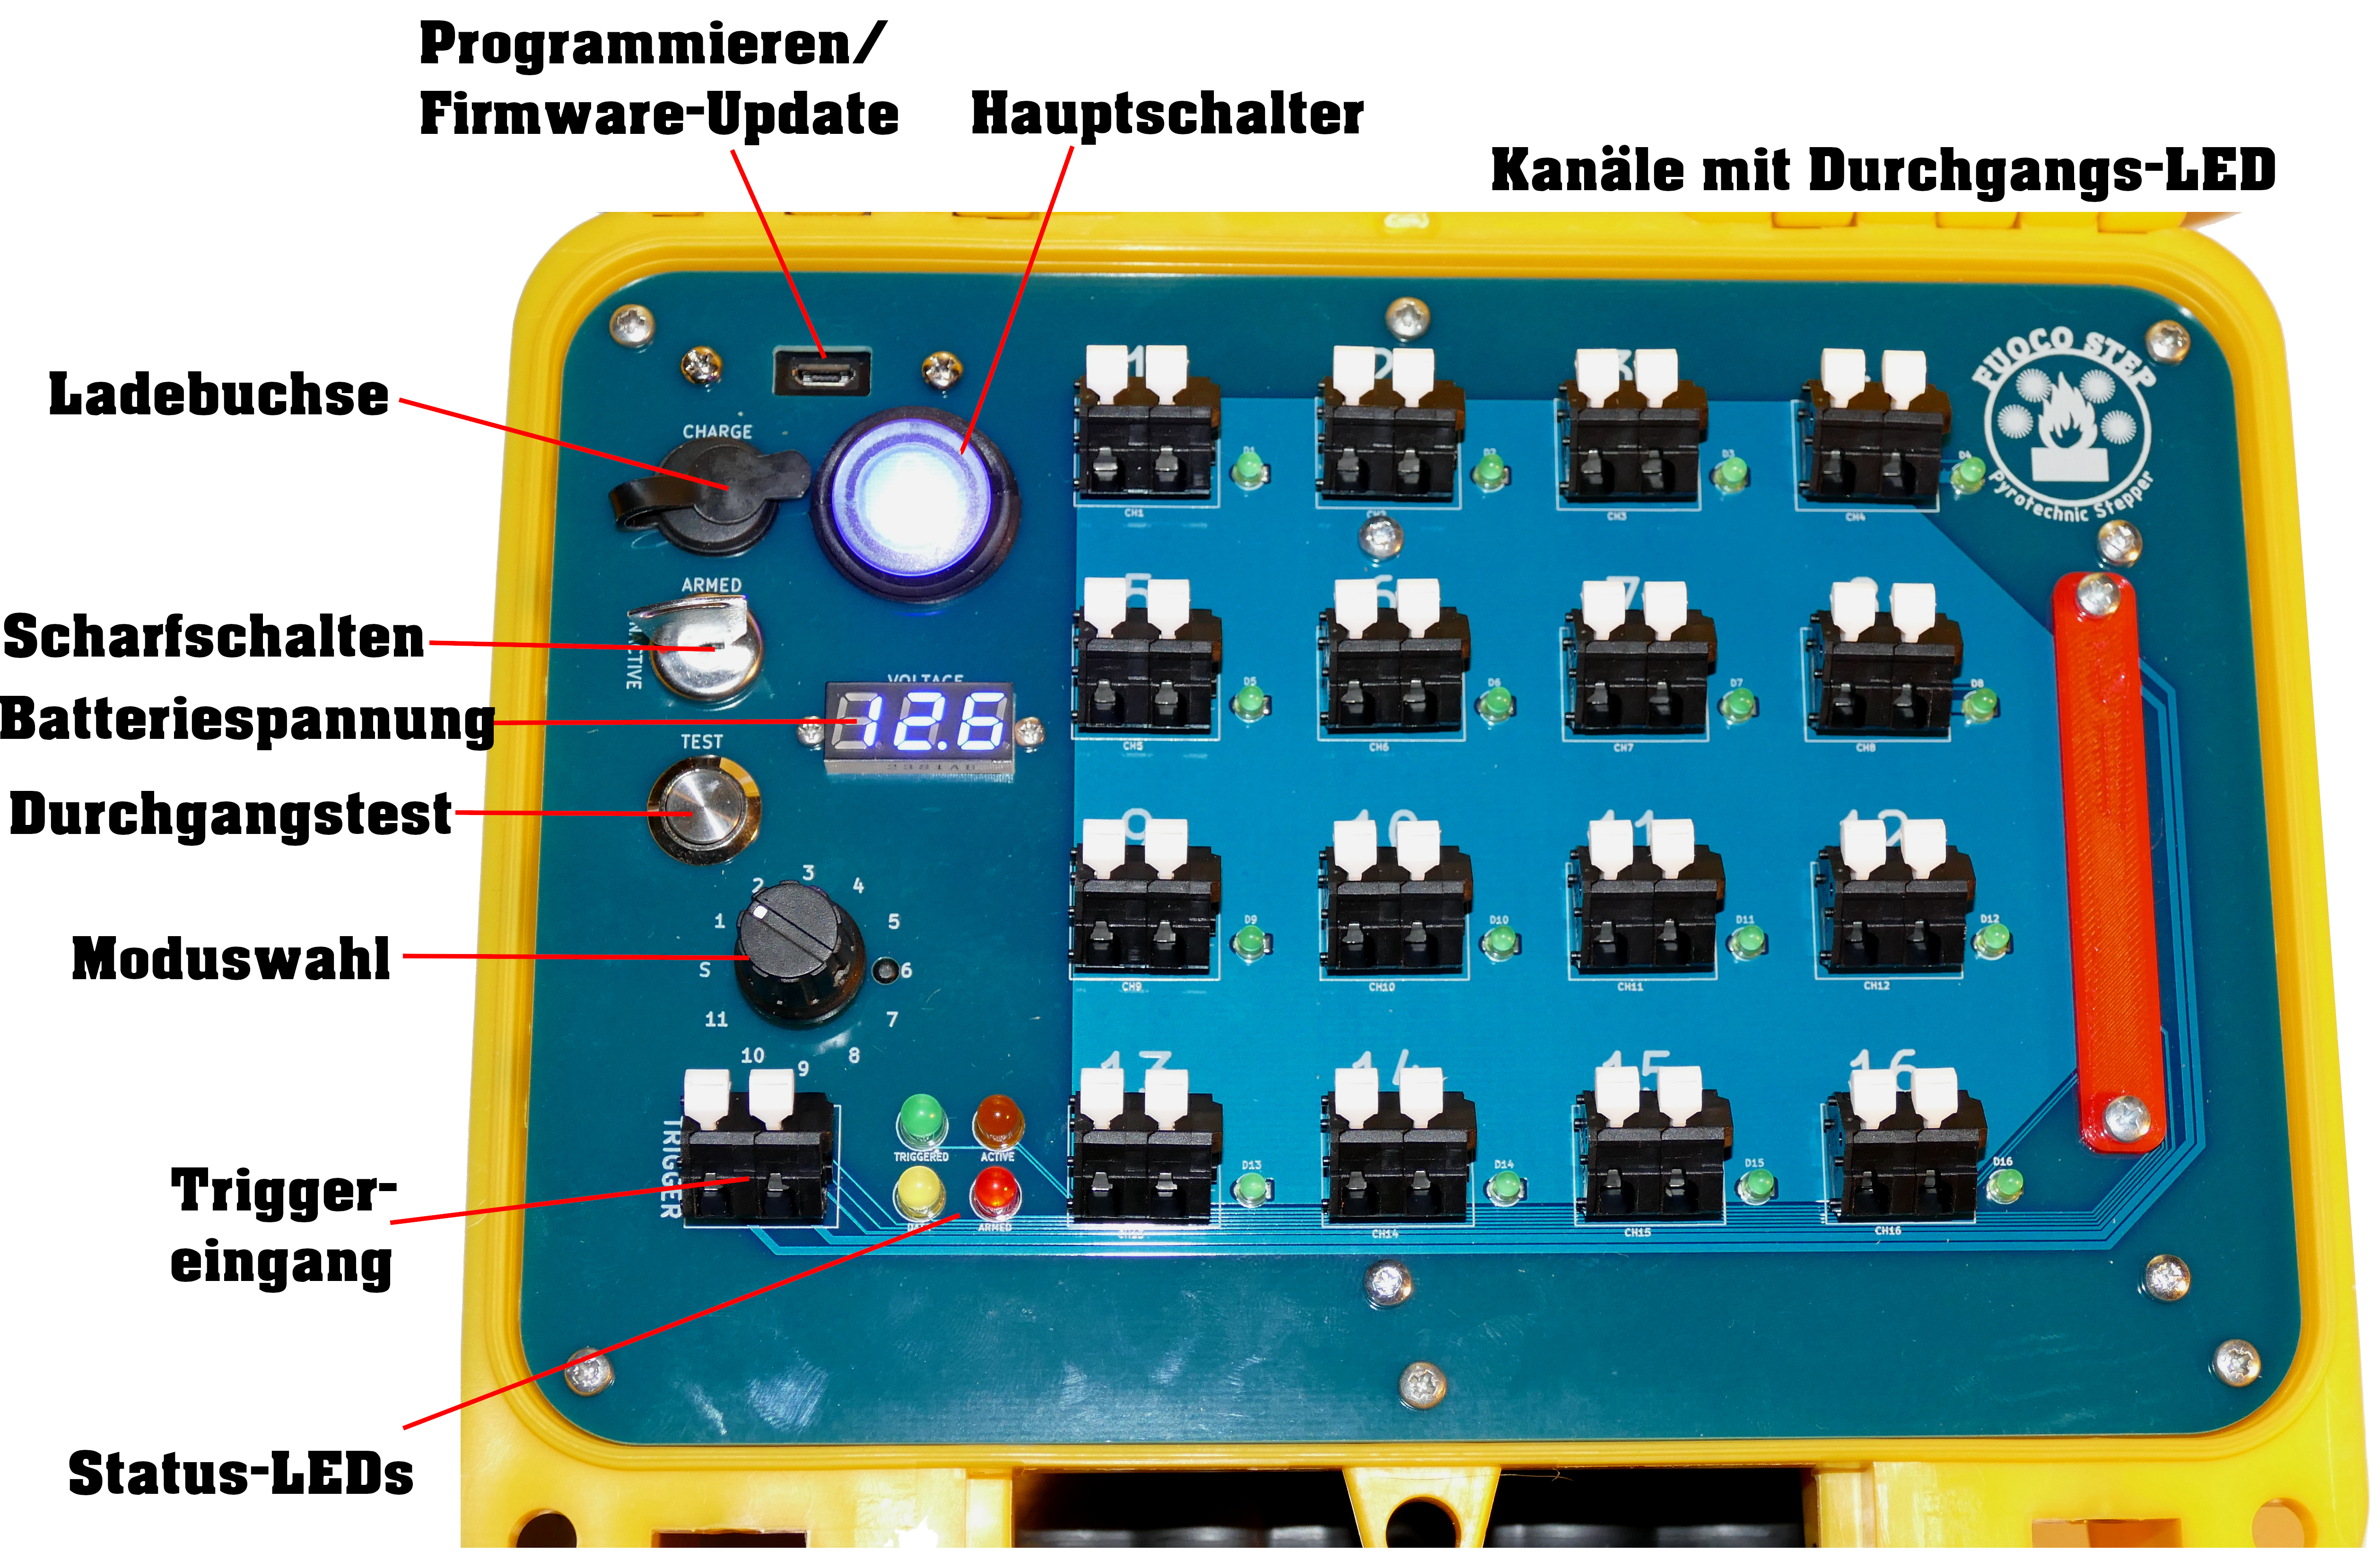
\includegraphics[width=\textwidth]{oberflaeche}
				\captionof{figure}{Übersicht über Bedienoberfläche}
				\label{fig:paneldescription}
			\end{center}

			Im einfachsten Modus fungiert das Device einfach als Portexpander, stellt also dem triggerenden Zündsystem zusätzliche Kanäle zur Verfügung, indem bei jedem Trigger ein Kanal ausgelöst wird. Beim ersten Aufruf des mit dem Trigger verbundenen Zündkanals wird dann Kanal 1 am Stepper gezündet, beim zweiten Kanal 2, usw.

			Zusätzlich können elf verschiedene Pattern im System hinterlegt werden, bei denen nach dem Trigger die Kanäle zeitgesteuert gezündet werden. Die möglichen Intervalle kann man auf Hundertstel genau zwischen 0,01 Sekunden und 9:59,99 Minuten festlegen. Es ist möglich, ein festes Intervall zwischen allen Kanälen zu nutzen, man kann aber auch jedes Intervall einzeln konfigurieren und hat sogar die Möglichkeit, die Sequenz bis zu einem erneuten Trigger zu unterbrechen. Die Wahl des aktuellen Patterns erfolgt über einen Drehschalter am Device, die Programmierung sowie eventuelle Firmwareupdates werden via PC, den man via Micro-USB-Kabel an den Stepper anschließt, erledigt. Hierzu kann ein simples Terminal-Programm wie PuTTy genutzt werden, ein graphisches User-Interface dazu existiert ebenfalls.

			Der Formfaktor des Geräts wurde für einen Seahorse-SE120-Koffer ausgelegt, Spannungsversorgung erfolgt über einen Blei-Gel-Akku (\SI{12}{\volt}/\SI{1,2}{\ampere\hour}), die Zündspannung beträgt 22,5 V, so dass auch längere Reihenschaltungen kein Problem darstellen. Der Triggereingang ist galvanisch vom Rest der Platine getrennt, eine gegenseitige Beeinflussung von Zündanlage und Stepper ist daher ausgeschlossen.

			Weiterhin existieren eine Spannungsanzeige zur Darstellung des aktuellen Batterieladestandes, ein Testschalter, um die Durchgangsprüfung der 16 Kanäle über die kleinen grünen LEDs darzustellen sowie ein Schlüsselschalter zum separaten Scharfschalten des Steppers. Der Akku kann über die integrierte Ladebuchse ohne Aufschrauben mit einem passenden Ladegerät für Blei-Gel-Akkus geladen werden.

			Die Bedienoberfläche unterteilt sich wie in Abbildung~\ref{fig:paneldescription} gezeigt. Auf die einzelnen Funktionen wird in den folgenden Abschnitten eingegangen.

			\section{Hauptschalter}

				Hiermit wird FUOCO STEP ein- und ausgeschaltet. Im eingeschalteten Zustand leuchtet die in den Schalter integrierte LED. Zu beachten ist, dass auch bei ausgeschaltetem Hauptschalter bei gleichzeitig verbundenem USB-Kabel der Logikteil des Steppers mit Strom versorgt, die Zündspannung aber nicht generiert wird. Für die Programmierung muss also der Hauptschalter nicht zwingend eingeschaltet sein.

			\section{Batterieanzeige}

				Bei eingeschaltetem Hauptschalter aktiviert sich die Spannungsanzeige und zeigt nach kurzer Wartezeit die gemessene Batteriespannung des Blei-Gel-Akkus an. Für einen stabilen Betrieb sollte der Wert stets im Bereich von \SI{12}{\volt} oder höher liegen, ansonsten sollte die Batterie nachgeladen werden.

			\section{Ladebuchse}

				Der innere Stift ist unmittelbar mit dem Pluspol des Akkus, der äußere Ring mit dem Minuspol des Akkus verbunden. Um das Ladegerät, z.B. ein H-TRONIC AL800, ungestört arbeiten zu lassen, sollte nur im ausgeschalteten Zustand geladen werden.

			\section{Durchgangstest}

				Ist dieser Schalter gedrückt, versucht die Anlage, einen geringen Strom, der sicher nicht zur Auslösung der Anzünder führt, auf allen Kanälen fließen zu lassen. Das Leuchten der zugehörigen grünen 3-mm-LED signalisiert, dass auf dem entsprechenden Kanal ein Strom fließen kann. Auf diese Weise können Kabelbrüche oder nicht-leitende Verbindungen detektiert werden, eine echte Widerstandsmessung des Kanals findet jedoch nicht statt. Der Testschalter hat keinen Einfluss auf den Zündvorgang, es kann also mit gedrücktem oder ungedrücktem Testschalter gezündet werden.

			\section{Scharfschalten}

				Als zusätzliche Sicherheitsmaßnahme muss der Stepper mit dem Schlüsselschalter separat scharfgeschaltet werden. Wenn das System scharf ist, wird dies durch die dauerhaft leuchtende rote Status-LED (Armed) signalisiert.

			\section{Modusauswahl}
				Der Drehschalter besitzt zwölf Positionen, den Single-Trigger-Modus \enquote{S} sowie die programmierbaren Positionen 1-11. Die Schalterposition wird erfasst, wenn der Schlüsselschalter auf scharf geschaltet wird, eine nachträgliche Drehung hat zunächst keine Wirkung. Über die Bedienoberfläche können jeweils für die aktuell eingestellte Drehschalterposition der Intervallmodus (fest/variabel) sowie die Intervallzeiten festgelegt werden. Näheres dazu in Kapitel~\ref{sec:gui}.

			\section{Triggereingang}
				Über diese Klemme wird der Stepper gestartet, sofern er zuvor scharfgeschaltet wurde. Die Polarität am Eingang spielt keine Rolle, das triggernde Gerät muss mindestens \SI{200}{\milli\ampere} über \SI{47}{\ohm} liefern können, um den Stepper auszulösen.

			\section{Kanalklemmen}
				Hier werden die Anzünder für die einzelnen Kanäle angeschlossen. Die Reihenfolge der Kanäle kann nicht beeinflusst werden, es wird also immer zuerst Kanal 1, dann Kanal 2, usw. ausgelöst. Aufgrund der Zündspannung von \SI{22,5}{\volt} sind längere Reihenschaltungen bis zu zehn Anzündern in Reihe pro Kanal möglich. Die rechts neben den Klemmen befindlichen LEDs signalisieren Durchgang auf dem jeweiligen Kanal, sofern der Testschalter gedrückt ist.

			\section{Status-LEDs}
				Diese vier LEDs signalisieren wesentliche Zustände des Systems.
				\begin{description}
					\item[Gelb/Data] Diese LED leuchtet, während Daten über USB mit dem Rechner ausgetauscht werden
					\item[Rot/Armed] Durch diese LED wird signalisiert, dass der Stepper scharfgeschaltet ist
					\item[Grün/Triggered] Diese LED zeigt an, dass das System getriggert wurde und aktuell eine Sequenz läuft
					\item[Orange/Active] Diese LED leuchtet, solange mindestens ein Kanal aktiv ist
				\end{description}

			\section{Programmieranschluss}
				Durch Anschließen eines Micro-USB-Kabels kann der Stepper über diese Schnittstelle programmiert werden. Dies ist im Detail im Kapitel~\ref{sec:gui} genau beschrieben. Auch Firmware-Updates sind über diesen Anschluss durchführbar.

		\chapter{Programmierung}
			\label{sec:gui}
			\section{Treiberinstallation}
				Idealerweise erkennt Windows beim Anschließen das Gerät (Microchip USB/UART Combo) von selbst und installiert den benötigten Treiber. Ansonsten muss über den Geräte-Manager der entsprechende Treiber manuell installiert werden.

			\section{Oberfläche}
				Über die Programmieroberfläche ist es möglich, die Steppereinstellungen zu modifizieren. Hierzu muss der passende COM-Port ausgewählt und zunächst die Einstellung des aktuell eingestellten Kanals ausgelesen werden.

				\begin{center}
					\includegraphics[width=.6\textwidth]{gui}
					\captionof{figure}{Übersicht über Bedienoberfläche}
					\label{fig:gui}
				\end{center}

				Bei Klick auf \enquote{Standardwerte wiederherstellen} werden \underline{alle} Kanäle zurückgesetzt auf festen Intervallmodus mit folgenden Intervallen:

				\begin{longtabu} [c]{S|S}
					{Schalterposition} & {Intervall (s)} \\ \hline\hline
					1                  & 2.5             \\
					2                  & 5.0             \\
					3                  & 7.5             \\
					4                  & 10.0            \\
					5                  & 12.5            \\
					6                  & 15.0            \\
					7                  & 17.5            \\
					8                  & 20.0            \\
					9                  & 25.0            \\
					10                 & 30.0            \\
					11                 & 40.0            \\ \hline
				\end{longtabu}

				Alle Änderungen die bei Schalterstellung \enquote{S} getätigt werden sollen, werden ignoriert.

				Das Zusatzfenster \enquote{Absolutzeiten} soll ein bequemes Umrechnen von absoluten Zündzeiten, wie man sie in einer Software wie PyroIgnitionControl festlegt, in die von FUOCO~STEP benötigten Intervallzeiten zwischen den einzelnen Kanälen ermöglichen. Hierzu können die Werte in der zweiten Spalte eingefügt und die Zeitabstände der einzelnen Kanäle durch Klick auf \enquote{Berechne Intervalle} ermittelt werden. Über \enquote{Werte ins Hauptfenster} können diese Intervallzeiten ins Hauptfenster übertragen werden. Dabei ist darauf zu achten, dass die aktuelle Schalterposition im passenden Modus konfiguriert sein muss. Ist der feste Intervallmodus eingestellt, wird nur der erste Intervallwert ins Hauptfenster kopiert, beim variablen Intervallmodus alle nicht-leeren Felder. Nach Übertragung ins Hauptfenster müssen die Werte noch durch \enquote{Intervalle setzen} ins Gerät geschrieben werden, um die berechneten Intervalle nutzen zu können.
\end{document}
